\documentclass[10pt,a4paper,twocolumn]{article}
\usepackage[margin=1.8cm,columnsep=0.7cm]{geometry}
\usepackage{booktabs}
\usepackage{graphicx}
\usepackage{xcolor}
\usepackage[hidelinks]{hyperref}
\usepackage{enumitem}
\usepackage{titlesec}
\usepackage{lmodern}
\usepackage[T1]{fontenc}
\usepackage{microtype}
\usepackage{parskip}
\usepackage{amsmath}
\usepackage{amssymb}
\usepackage{caption}
\usepackage{abstract}

\captionsetup{font=small,labelfont=bf,skip=4pt}
\setlength{\abovecaptionskip}{4pt}
\titlespacing*{\section}{0pt}{6pt}{3pt}
\titlespacing*{\subsection}{0pt}{5pt}{2pt}
\titleformat{\section}{\normalsize\bfseries}{\thesection}{0.5em}{}
\titleformat{\subsection}{\small\bfseries}{\thesubsection}{0.5em}{}
\setlength{\parskip}{2pt}
\setlength{\absleftindent}{0pt}\setlength{\absrightindent}{0pt}
\renewcommand{\abstractnamefont}{\normalfont\bfseries\small}
\renewcommand{\abstracttextfont}{\normalfont\small}

\newcommand{\kf}[1]{\vspace{1pt}\noindent\fcolorbox{black!35}{black!5}{%
  \parbox{0.955\linewidth}{\small\vspace{1pt}#1\vspace{1pt}}}\vspace{3pt}}

\title{\vspace{-1.4cm}\textbf{\large A Longitudinal, Subject-Coherent Journal
from Knesset Committee Protocols}\\[3pt]
\normalsize\normalfont Segmentation, Streaming Subject Linking, and Context-Conditioned Log Writing}
\author{\small Tomer Morad \quad Or Israeli \quad Yoel Marko \\[1pt]
\small\textit{Advanced NLP (ANLP), July 2026}}
\date{}

\begin{document}
\twocolumn[
\begin{@twocolumnfalse}
\maketitle
\vspace{0.15cm}
\begin{abstract}
\noindent We build a longitudinal journal over a stream of Israeli Knesset Finance Committee
transcripts, coupling three tasks --- topic segmentation, \emph{streaming} cross-document
subject linking, and update summarization --- under an asymmetric cost model in which false
merges are worse than false splits. Our central result is negative and, we argue, the most
useful thing the project produced. On a manually annotated gold set of 523 segments, one fixed
representation (\texttt{multilingual-e5-large}+ABTT) scores $F_1{=}0.619$ judging subject
identity over \emph{pairs}, and $F_1{=}0.125$ when the \emph{same representation} makes the
\emph{same decision} online against a growing journal. The collapse is not caused by weak
embeddings but by the structure of the streaming decision, where only $6.9\%$ of arrivals are
true repeats. We show what closes the gap --- an accumulated-centroid entry representation
lifts recall $32\%{\to}89\%$, and a distinctiveness \emph{margin} rule raises $F_1$
$0.103{\to}0.190$ --- while every LLM verifier we tried stays $\le 0.111$. We further document
two ways this benchmark silently rewards look-ahead, and report all headline numbers under a
streaming-honest protocol.
\end{abstract}
\vspace{0.35cm}
\end{@twocolumnfalse}]

\section{Introduction}

A Knesset committee returns to the same legislative matter repeatedly over months, so
reconstructing the history of one matter means reading dozens of unrelated transcripts. We
aim to produce that history automatically: an index in which each entry is one underlying
matter carrying a dated log of its progress. This decomposes into (i) partitioning each
protocol into subject spans, (ii) deciding online whether a new span continues an existing
entry or opens a new one, and (iii) generating only the \emph{incremental} update.

\textbf{Asymmetric cost.} Merging two distinct matters corrupts an entry permanently and
silently; splitting one matter is visible and repairable. We therefore report every operating
point twice: at best $F_1$, and at the \emph{anti-duplication} point where the false-merge
rate (FMR) is held $\le 5\%$.

\textbf{Research question.} \emph{Why does near-ceiling subject separability fail to produce
usable streaming linking, and what closes the gap?} Our contributions: a gold standard over
211/213 protocols (\S\ref{sec:data}); a quantification of the separability/decision gap
(\S\ref{sec:gap}); an analysis of which levers close it (\S\ref{sec:levers}); evidence the LLM
helps as an \emph{extractor} not a \emph{classifier} (\S\ref{sec:llm}); two look-ahead leaks
and an honest protocol (\S\ref{sec:honesty}); and a diagnosis of update summarization's
recap-then-append failure (\S\ref{sec:log}).

\section{Data and Gold Standard}
\label{sec:data}

We use 213 Hebrew transcripts from the 25th Knesset Finance Committee. Protocol-level subject
markers yield 151 canonical topics after fuzzy variant merging, but these describe the
\emph{meeting}, not the spans inside it, so we manually segmented 211/213 protocols:

\begin{center}\small
\begin{tabular}{lr}
\toprule
Gold segments (subject spans) & 523 \\
Distinct subject labels & 487 \\
Recurring matters ($\ge 2$ appearances) & 22 \\
Repeat events (decidable link decisions) & 36 \\
Base rate of repeats among arrivals & $6.9\%$ \\
\bottomrule
\end{tabular}
\end{center}

We deliberately did \emph{not} merge near-duplicate labels across protocols: under the
asymmetric cost rule an unmerged duplicate is a cheap false split, whereas an incorrect merge
would corrupt the gold itself. Recurrence counts are therefore conservative.

\section{Segment Representation}

Using only discussion \emph{content} (no headers, agendas, attendees or speaker names), do
segments of one matter cluster together? Off-the-shelf dense encoders are severely
anisotropic: cross-topic cosine averages $\approx0.95$, leaving a same/different gap of
$0.007$--$0.066$, and under those conditions TF-IDF beat every dense model because the
discriminative signal is lexical (bill numbers, entities). All-But-The-Top (ABTT) --- centering
and projecting out the top-$k$ principal directions, which encode register rather than
subject --- reverses this.

\begin{center}\small
\begin{tabular}{lcc}
\toprule
Representation & ARI (agg.) & Pairwise AUC \\
\midrule
e5, no ABTT ($k{=}0$) & 0.124 & 0.857 \\
\textbf{e5 + ABTT ($k{=}1$)} & \textbf{0.657} & \textbf{0.954} \\
TF-IDF & 0.382 & 0.874 \\
AlephBERT + ABTT ($k{=}2$) & 0.265 & 0.854 \\
\bottomrule
\end{tabular}
\end{center}

\kf{\textbf{Encoder choice matters, but de-anisotropization matters more.} Removing a
\emph{single} direction moves e5 from ARI $0.124$ to $0.657$ --- a larger effect than the
spread across e5, TF-IDF and AlephBERT combined. We fix \texttt{e5+ABTT-$k$1} for all
subsequent experiments.}

\section{Streaming Subject Linking}

\subsection{The separability/decision gap}
\label{sec:gap}

We evaluate one representation under two protocols: \textbf{pairwise}, scoring all segment
pairs (measuring \emph{separability}, with oracle access to the full set), and
\textbf{streaming}, where segments arrive chronologically and each is scored against the
journal built so far --- the actual task.

\begin{center}\small
\begin{tabular}{lccccc}
\toprule
Protocol & AUC & $F_1$ & P & R & FMR \\
\midrule
Pairwise (oracle) & 0.954 & \textbf{0.619} & 0.500 & 0.811 & 0.038 \\
Streaming (real) & --- & \textbf{0.125} & 0.077 & 0.333 & 0.296 \\
\bottomrule
\end{tabular}
\end{center}

\kf{\textbf{Central result.} A representation separating same- from different-matter pairs at
$F_1\,0.619$ collapses to $F_1\,0.125$ when the same decision is made online.
\textbf{The bottleneck is the streaming decision structure, not representation quality.}}

\textbf{Why.} Only 36 of 523 arrivals are repeats. Each is compared against a journal growing
toward several hundred entries, so with $n$ candidates expected false merges scale as
$n\cdot\mathrm{FPR}$ while available true positives stay at most one. A false-positive rate
low enough to look excellent pairwise still floods the true matches --- a base-rate effect,
and precisely what makes anti-duplication hard. Notably, \textbf{retrieval was never the
bottleneck}: similarity ranking places the correct entry in the top 10 for \emph{all} 36
repeats (recall@1 $0.694$, @5 $0.944$, @10 $1.000$). The information is in the shortlist; the
\emph{decision} fails.

\begin{figure}[t]
\centering
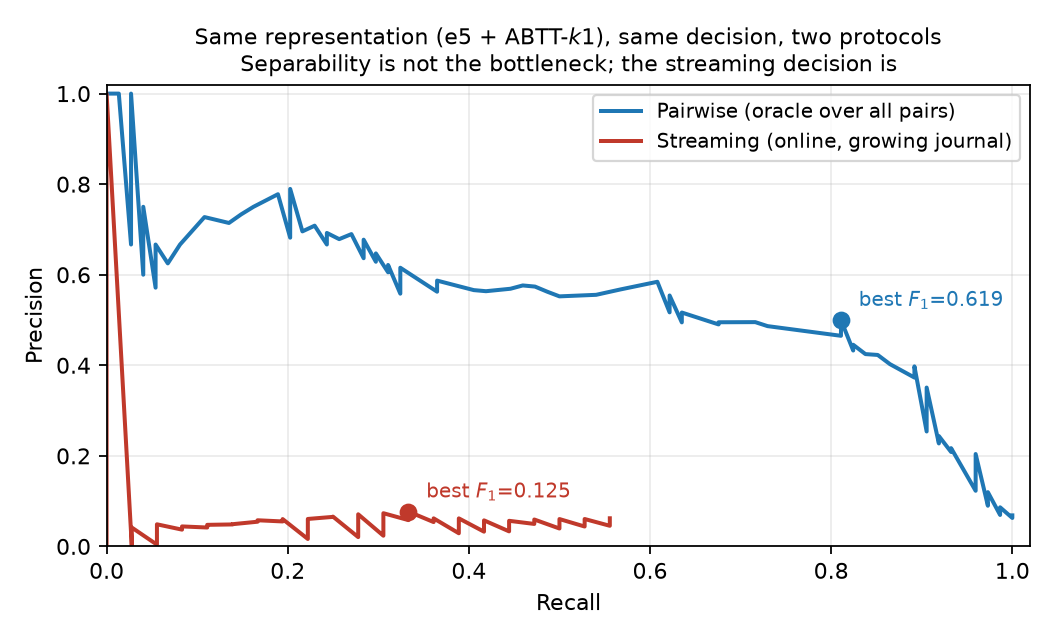
\includegraphics[width=\linewidth]{fig_gap.png}
\vspace{-14pt}
\caption{Precision--recall for one representation under both protocols. The oracle frontier
sustains precision near $0.6$; the streaming frontier never exceeds $\approx0.08$. The area
between them is attributable to the decision setting, not the embedding.}
\label{fig:gap}
\end{figure}

\subsection{What closes the gap}
\label{sec:levers}

From a baseline representing each entry by its frozen first span and linking above a cosine
threshold, we vary one component at a time on frozen embeddings, CPU-only.

\begin{center}\small
\begin{tabular}{lcc}
\toprule
Method (streaming-honest) & $F_1$ & R @ FMR$\le5\%$ \\
\midrule
Baseline: first span + threshold & 0.103 & $2.8\%$ \\
\ \ + accumulated centroid & --- & R $32\%{\to}89\%$ \\
\ \ + distinctiveness margin & \textbf{0.190} & $\mathbf{8.6\%}$ \\
\midrule
Best LLM verifier (snippet) & 0.111 & $\approx0\%$ \\
LLM verifier, full timeline & 0.068 & $0\%$ \\
\bottomrule
\end{tabular}
\end{center}

\textbf{Represent the matter, not its first span.} Replacing the frozen first span with the
running centroid of an entry's members lifts recall $32\%\to89\%$: the streaming setting
continuously supplies evidence about what a matter looks like, and the baseline discards it.

\textbf{Distinctiveness beats magnitude.} Instead of ``is the best candidate similar enough?''
($\cos\ge\theta$), the margin rule asks ``is it \emph{distinctly} more similar than the
runner-up?'' ($\cos_{(1)}-\cos_{(2)}\ge\theta$). This targets the real failure mode: the corpus
contains families of near-identical bureaucratic templates, so high absolute similarity is
uninformative while a large \emph{gap} is not.

\subsection{Extractor, not classifier}
\label{sec:llm}

As a \textbf{verifier} deciding same/related/new from a candidate snippet, the LLM reached
$F_1\,0.111$; given the candidate's \emph{full accumulated timeline} --- the retrieve-then-verify
design --- it got \emph{worse} ($0.068$), the longer context increasing its willingness to
merge. As an \textbf{extractor} producing stable matter fingerprints (laws, programmes,
entities) fused additively with the geometric score it helped: under a common batch-fit
setting, geometry alone $0.200$ vs.\ geometry+fingerprints $0.241$ (\texttt{dictalm2}) and
$0.201$ (\texttt{qwen7b}).

\kf{Every LLM \emph{classifier} variant scored at or below the CPU-only geometric method. The
LLM's value was in \emph{extracting stable identifiers}, leaving the decision to geometry.}

\subsection{Two look-ahead leaks}
\label{sec:honesty}

Streaming benchmarks make it easy to use future information unnoticed; we found two instances
in our own pipeline. \textbf{(1) Batch-fit transforms.} ABTT and whitening estimate parameters
from the embedding matrix; fitting once over the whole corpus uses segments that have not yet
arrived. Refit honestly at each step from the observed prefix, the apparently strongest
configuration collapses.

\begin{center}\small
\begin{tabular}{lcc}
\toprule
Transform & Batch (leaky) & Honest refit \\
\midrule
Whitening (50-dim) & 0.250 & 0.094 \\
Centering & 0.175 & 0.190 \\
ABTT-$k$1 & 0.200 & 0.162 \\
\bottomrule
\end{tabular}
\end{center}

Whitening needs a 50-dimensional covariance estimate that does not exist early in the stream;
cheap transforms needing few samples survive, expensive ones do not. \textbf{(2) Undefined
cold-start margins.} With exactly one journal entry the runner-up is undefined; substituting a
sentinel $-1$ makes the margin $\cos+1$, clearing any threshold, so the second segment of every
run merges unconditionally. The correct fallback is the raw similarity magnitude.

\kf{Several configurations look like improvements under batch fitting and are partly
measurement artifacts. \textbf{On streaming benchmarks the fitting protocol must be reported
alongside the metric.}}

\section{Context-Conditioned Log Writing}
\label{sec:log}

Each update is conditioned on the running journal built from the model's \emph{own} prior
generations (faithfulness is chain-relative). Because predicted links are only $\approx13\%$
precise, evaluating through them would conflate two failures; we therefore evaluate on
\textbf{gold chains} (22 matters, 58 entries), judged by a third model that is neither
generator.

\begin{center}\small
\begin{tabular}{lcccc}
\toprule
& \multicolumn{2}{c}{\texttt{dictalm2}} & \multicolumn{2}{c}{\texttt{qwen2.5-7b}} \\
\cmidrule(lr){2-3}\cmidrule(lr){4-5}
Prompt & Faith. & Nov. & Faith. & Nov. \\
\midrule
Zero-shot & \textbf{80.7} & \textbf{18.1} & 63.4 & \textbf{10.1} \\
+ example (real) & 71.1 & 15.0 & 63.1 & 8.3 \\
+ example (fictional) & 53.6 & 5.0 & \textbf{69.2} & 5.3 \\
\bottomrule
\end{tabular}
\end{center}

Faithfulness is acceptable --- the Hebrew-native \texttt{dictalm2} is clearly more grounded
than the stronger general-purpose model --- but novelty is the failure. Rather than emitting a
pure diff, models re-establish context around whatever new fact they add, so even the best
examples reach only $\approx50/100$; an explicit ``do not repeat what is already logged''
instruction does not prevent it.

\kf{\textbf{Few-shot prompting made this monotonically worse for both models}
($18.1{\to}15.0{\to}5.0$; $10.1{\to}8.3{\to}5.3$). In the worst condition $92\%$ of updates
were near-verbatim copies of the example's answer: for a free-text \emph{incremental-diff}
task, examples are imitated as \emph{content} rather than \emph{style} --- the opposite of the
classification task in \S\ref{sec:llm}.}

\section{End-to-End Pipeline and Canonicalization}

Composed end-to-end (embed $\to$ link $\to$ write) on all 523 gold segments under predicted
growth, the anti-duplication operating point ($\theta{=}0.342$) yields 493 entries of which 23
are multi-session, at $0.954$ purity; the best-$F_1$ point ($\theta{=}0.156$) yields 329 entries,
76 multi-session, at $0.658$ purity. We treat this journal as a \emph{demonstration artifact},
not an evaluation surface: at $0.13$ linking precision an end-to-end score would conflate
linking with summarization error, so each task is evaluated against gold inputs.

A parallel line of work in our group rewrites segments into neutral third-person Hebrew before
embedding, targeting exactly the register confound of \S\ref{sec:levers}. On 19 protocols it
sharpened intrinsic separation (substantive-segment AUC $0.947\to0.986$) but inverted
downstream: $F_1$ $0.114\to0.095$, with precision $0.073\to0.154$ and recall $0.261\to0.069$.
It roughly doubles precision while collapsing recall --- which under our asymmetric cost model
is the \emph{desirable} direction even though $F_1$ falls, meaning $F_1$ is the wrong
instrument here. Two caveats prevent a stronger claim: the pseudo-labels come from the same LLM
pass that produced the canonical text, and 29 repeat events is too thin to move $F_1$ stably.

\section{Limitations and Conclusion}

36 repeat events is few: recall at FMR$\le5\%$ moves in $2.8$-point increments, so large
effects (representation, decision rule) are safe conclusions while fine rankings are not.
Segmentation is gold rather than predicted, so an automatic segmenter would add its own error.
All results come from one committee whose budget proceedings are unusually templated, and
log-writing scores come from a 3B judge.

The intuitive failure mode --- ``Hebrew embeddings are not good enough'' --- is not what we
found: a CPU-side representation separates same- from different-matter segments at AUC $0.954$.
What defeats the system is the streaming decision itself, where a $6.9\%$ base rate against a
growing candidate set means an excellent false-positive rate still produces more false merges
than true ones. Consistent with that diagnosis, the levers that helped were structural rather
than representational --- represent the accumulated matter rather than its first appearance,
and judge \emph{distinctiveness} rather than \emph{similarity} --- while larger models in the
deciding role did not help at all.

\vspace{2pt}
{\footnotesize\noindent\textbf{Reproducibility.} The project is organised as numbered,
self-contained steps (\texttt{steps/01..13}), each with its own \texttt{code/},
\texttt{outputs/} and \texttt{README.md}. Every number and figure traces to a committed JSON
artifact under \texttt{steps/*/outputs/}; Fig.~\ref{fig:gap} is regenerated by
\texttt{report/make\_report\_figs.py} with no hard-coded values.}

\end{document}
